% !TEX program = lualatex
% !BIB program = bibtex
% =========================================================================
% main.tex
% Plantilla de Informe de Prácticas Pre Profesionales (PPP)
% Universidad Nacional Agraria de la Selva (UNAS)
% Motor Tipográfico Exclusivo: LuaLaTeX
% =========================================================================
\documentclass{unas-ppp}

% 1. Cargar Metadatos del Documento y Opciones de Visibilidad
% =========================================================================
% config/metadata.tex
% Metadatos del Informe de Prácticas Pre Profesionales (UNAS)
% =========================================================================
% Este archivo es la ÚNICA FUENTE DE VERDAD para los datos del informe.
% Modifique los valores entre llaves con la información correspondiente.

% --- Datos Institucionales de la UNAS ---
\universidad{UNIVERSIDAD NACIONAL AGRARIA DE LA SELVA}
\facultad{FACULTAD DE INGENIERÍA EN INFORMÁTICA Y SISTEMAS}
\escuela{ESCUELA PROFESIONAL DE INGENIERÍA EN INFORMÁTICA Y SISTEMAS}

% --- Título del Informe ---
% Debe ser sintético, reflejar la labor desarrollada y concordar con el plan de prácticas.
\titulo{DESARROLLO DE UN SISTEMA DE INFORMACIÓN WEB PARA LA GESTIÓN OPERATIVA Y CONTROL DE PROCESOS}

% --- Datos del Practicante ---
% Nombres y apellidos completos según matrícula universitaria.
\autor{Nombres y Apellidos del Estudiante}

% --- Asesor Académico ---
% Grado académico y nombre completo del docente asesor asignado por la facultad.
\asesor{Ing. Nombre y Apellidos del Asesor, Mg.}

% --- Periodo de Ejecución ---
% Formato: DD/MM/AAAA al DD/MM/AAAA (Debe cubrir las horas reglamentarias).
\periodo{01/01/2026 al 31/03/2026}

% --- Entidad Receptora de las Prácticas ---
% Razón social o denominación de la empresa o institución donde se realizaron las PPP.
\empresa{EMPRESA O INSTITUCIÓN RECEPTORA S.A.C.}

% --- Lugar y Fecha de Publicación ---
\ciudad{TINGO MARÍA}
\pais{PERÚ}
\anio{2026}

% --- Rutas de los Logos Institucionales ---
% Por defecto utiliza los logos oficiales en assets/logos/
\logoUniversidad{assets/logos/unas.png}
\logoFacultad{assets/logos/fiis_unas.jpg}

% =========================================================================
% config/opciones.tex
% Configuración de Visibilidad y Banderas Booleanas del Documento
% =========================================================================
% Active (true) o desactive (false) los componentes según la etapa de su informe:
% - Durante elaboración/revisión: mantener mostrarActa en false.
% - Tras la sustentación final: activar mostrarActa y mostrarQR si corresponde.

% Aviso de código QR institucional (se incluye tras levantamiento de observaciones)
\newbool{mostrarQR}
\setbool{mostrarQR}{false}

% Dictamen favorable del asesor docente
\newbool{mostrarDictamen}
\setbool{mostrarDictamen}{true}

% Certificado o constancia de prácticas emitida por la empresa
\newbool{mostrarConstancia}
\setbool{mostrarConstancia}{true}

% Acta de exposición y sustentación ante el jurado calificador
\newbool{mostrarActa}
\setbool{mostrarActa}{false}

% Página de Dedicatoria (opcional según el estudiante)
\newbool{mostrarDedicatoria}
\setbool{mostrarDedicatoria}{true}

% Página de Agradecimientos (opcional según el estudiante)
\newbool{mostrarAgradecimientos}
\setbool{mostrarAgradecimientos}{true}

% Generación de Índices Auxiliares
\newbool{mostrarIndiceTablas}
\setbool{mostrarIndiceTablas}{true}

\newbool{mostrarIndiceFiguras}
\setbool{mostrarIndiceFiguras}{true}


\begin{document}

% 2. Portada Reglamentaria UNAS
\makecaratula

% 3. Secciones Preliminares (Modulares y Condicionales)
\iniciarpreliminares
% =========================================================================
% preliminares/00_qr_aviso.tex
% Aviso institucional para código QR
% =========================================================================
\ifbool{mostrarQR}{%
  \clearpage
  \thispagestyle{empty}
  \vspace*{7cm}
  \begin{center}
    \fontsize{12pt}{14pt}\selectfont
    \textit{\{El código QR de verificación institucional se incluirá tras la sustentación\\ y el respectivo levantamiento de observaciones aprobadas por el jurado\}}
  \end{center}
  \vfill
  \clearpage
}{}

% =========================================================================
% preliminares/01_dictamen.tex
% Dictamen de Aprobación del Docente Asesor
% =========================================================================
\ifbool{mostrarDictamen}{%
  \clearpage
  \thispagestyle{empty}
  \IfFileExists{assets/documentos/dictamen_asesor.pdf}{%
    \includepdf[pages=-]{assets/documentos/dictamen_asesor.pdf}%
  }{%
    \IfFileExists{assets/documentos/dictamen_asesor.png}{%
      \vspace*{\fill}%
      \begin{center}%
        \makebox[\textwidth][c]{\includegraphics[width=0.95\textwidth]{assets/documentos/dictamen_asesor.png}}%
      \end{center}%
      \vspace*{\fill}%
    }{%
      \vspace*{5cm}%
      \begin{center}%
        \fbox{%
          \parbox{0.85\textwidth}{%
            \centering\vspace{1cm}%
            \textbf{\large DICTAMEN DEL DOCENTE ASESOR}\\[0.5cm]%
            \textit{Coloque el archivo escaneado o digital del dictamen firmado en:}\\[0.3cm]%
            \texttt{assets/documentos/dictamen\_asesor.pdf}\\[0.2cm]%
            o en formato imagen \texttt{.png / .jpg}.%
            \vspace{1cm}%
          }%
        }%
      \end{center}%
      \vfill%
    }%
  }%
  \clearpage
}{}

% =========================================================================
% preliminares/02_constancia.tex
% Certificado / Constancia de Prácticas Emitida por la Empresa
% =========================================================================
\ifbool{mostrarConstancia}{%
    \clearpage
    \thispagestyle{empty}
    \IfFileExists{assets/documentos/constancia_practicas.pdf}{%
        \includepdf[pages=-]{assets/documentos/constancia_practicas.pdf}%
    }{%
        \IfFileExists{assets/documentos/constancia_practicas.png}{%
            \vspace*{\fill}%
            \begin{center}%
                \makebox[\textwidth][c]{\includegraphics[width=0.95\textwidth]{assets/documentos/constancia_practicas.png}}%
            \end{center}%
            \vspace*{\fill}%
        }{%
            \vspace*{5cm}%
            \begin{center}%
                \fbox{%
                    \parbox{0.85\textwidth}{%
                        \centering\vspace{1cm}%
                        \textbf{\large CONSTANCIA / CERTIFICADO DE PRÁCTICAS}\\[0.5cm]%
                        \textit{Coloque el documento emitido por la empresa o institución en:}\\[0.3cm]%
                        \texttt{assets/documentos/constancia\_practicas.pdf}\\[0.2cm]%
                        o en formato imagen \texttt{.png / .jpg}.%
                        \vspace{1cm}%
                    }%
                }%
            \end{center}%
            \vfill%
        }%
    }%
    \clearpage
}{}

% =========================================================================
% preliminares/03_acta.tex
% Acta de Exposición y Sustentación
% =========================================================================
\ifbool{mostrarActa}{%
  \clearpage
  \thispagestyle{empty}
  \IfFileExists{assets/documentos/acta_sustentacion.pdf}{%
    \includepdf[pages=-]{assets/documentos/acta_sustentacion.pdf}%
  }{%
    \IfFileExists{assets/documentos/acta_sustentacion.png}{%
      \vspace*{\fill}%
      \begin{center}%
        \makebox[\textwidth][c]{\includegraphics[width=0.95\textwidth]{assets/documentos/acta_sustentacion.png}}%
      \end{center}%
      \vspace*{\fill}%
    }{%
      \vspace*{5cm}%
      \begin{center}%
        \fbox{%
          \parbox{0.85\textwidth}{%
            \centering\vspace{1cm}%
            \textbf{\large ACTA DE EXPOSICIÓN Y SUSTENTACIÓN}\\[0.5cm]%
            \textit{Coloque el acta firmada por el jurado evaluador en:}\\[0.3cm]%
            \texttt{assets/documentos/acta\_sustentacion.pdf}\\[0.2cm]%
            o en formato imagen \texttt{.png / .jpg}.%
            \vspace{1cm}%
          }%
        }%
      \end{center}%
      \vfill%
    }%
  }%
  \clearpage
}{}

% =========================================================================
% preliminares/04_dedicatoria.tex
% Página de Dedicatoria (Opcional)
% =========================================================================
\ifbool{mostrarDedicatoria}{%
  \clearpage
  \thispagestyle{empty}
  \vspace*{4cm}
  \begin{flushright}
    {\fontsize{12pt}{14pt}\selectfont\bfseries DEDICATORIA} \\[0.5cm]
    \parbox{0.65\textwidth}{%
      \raggedleft\itshape
      A mis padres y familiares, por su apoyo constante, sacrificio y motivación incondicional a lo largo de toda mi formación universitaria y personal.\\[0.3cm]
      A mis docentes y mentores del área técnica, por compartir sus conocimientos y orientarme durante el desarrollo de mis prácticas preprofesionales.
    }
  \end{flushright}
  \vfill
  \clearpage
}{}

% =========================================================================
% preliminares/05_agradecimientos.tex
% Página de Agradecimientos (Opcional)
% =========================================================================
\ifbool{mostrarAgradecimientos}{%
  \clearpage
  \thispagestyle{empty}
  \vspace*{4cm}
  \begin{flushright}
    {\fontsize{12pt}{14pt}\selectfont\bfseries AGRADECIMIENTOS} \\[0.5cm]
    \parbox{0.65\textwidth}{%
      \raggedleft\itshape
      A la Universidad Nacional Agraria de la Selva, por brindarme la formación profesional e integral en las aulas de estudio.\\[0.3cm]
      A la empresa receptora de prácticas y al equipo técnico del área, por abrirme sus puertas y otorgarme la confianza para ejecutar las actividades asignadas.\\[0.3cm]
      A mi asesor de prácticas, por sus oportunas revisiones y recomendaciones metodológicas.
    }
  \end{flushright}
  \vfill
  \clearpage
}{}

% =========================================================================
% preliminares/06_resumen.tex
% Resumen Ejecutivo y Palabras Clave
% =========================================================================
\clearpage
\thispagestyle{empty}

\begin{center}
  {\fontsize{14pt}{16pt}\selectfont\bfseries RESUMEN}
\end{center}
\vspace{0.5cm}

\fontsize{12pt}{14pt}\selectfont
El presente informe de prácticas preprofesionales describe el desarrollo y ejecución de actividades técnicas orientadas a resolver una problemática operativa en la institución receptora. En primer lugar, se describe la situación inicial y las limitaciones identificadas que motivaron la intervención. Posteriormente, se plantea el objetivo principal y los objetivos específicos orientados a diseñar, implementar y validar una solución robusta y estandarizada. Para alcanzar dichos propósitos, se aplicó una metodología de trabajo ágil estructurada en iteraciones periódicas, complementada con el uso de herramientas modernas de desarrollo de software, modelado de datos y aseguramiento de la calidad. Como resultado de las labores ejecutadas, se logró implementar con éxito los módulos funcionales requeridos, optimizando los flujos de trabajo internos y garantizando la estabilidad operativa del entorno. Finalmente, se concluye que la aplicación de principios de diseño y buenas prácticas de ingeniería permitió elevar significativamente la mantenibilidad, escalabilidad y eficiencia de los procesos en la organización.

\vspace{0.8cm}
\noindent\textbf{Palabras clave:} Prácticas preprofesionales, ingeniería de software, arquitectura de sistemas, optimización de procesos, desarrollo web.
\clearpage


% 4. Índices Automáticos (Contenido, Tablas y Figuras)
\makepreliminares

% 5. Cuerpo del Informe (Inicia numeración arábiga en página 1)
\iniciarcuerpo
% =========================================================================
% capitulos/01_aspectos_generales.tex
% Capítulo I: Introducción y Aspectos Generales de la Entidad
% =========================================================================

\section*{INTRODUCCIÓN}
\addcontentsline{toc}{section}{INTRODUCCIÓN}

La introducción debe presentar de manera clara y concisa el propósito del informe de prácticas preprofesionales, contextualizando el entorno en el que se llevaron a cabo las actividades. Se recomienda exponer brevemente la necesidad técnica o empresarial identificada en la institución receptora, el enfoque de ingeniería o metodología adoptado para su atención y los resultados principales alcanzados durante el periodo asignado.

Asimismo, es conveniente sintetizar la organización del documento indicando el contenido medular de cada uno de los capítulos: el Capítulo I comprende la descripción y aspectos generales de la entidad receptora; el Capítulo II expone el marco teórico y tecnológico de soporte; el Capítulo III detalla las actividades técnicas realizadas, objetivos, metodología y desarrollo; y finalmente, se presentan las conclusiones y recomendaciones derivadas de la experiencia profesional.

\section{Aspectos Generales de la Entidad}

\subsection{Información general de la institución}

\subsubsection{Identificación de la institución}
Describa la razón social, tipo de personería jurídica (pública o privada), número de Registro Único de Contribuyentes (RUC) y el rubro general de operaciones de la empresa o institución donde se ejecutaron las prácticas preprofesionales.

\subsubsection{Ubicación de la institución}
Indique la dirección física exacta de la sede u oficina principal (distrito, provincia y departamento). De ser pertinente, mencione las sucursales, portales web corporativos y canales oficiales de comunicación institucional.

\subsubsection{Misión y Visión}
\textbf{Misión:} \\
Describa la misión institucional establecida por la entidad receptora, enfocándose en su razón de ser, público objetivo y propuesta de valor en el mercado o sector en el que opera.

\vspace{0.3cm}
\textbf{Visión:} \\
Presente la visión estratégica de la entidad, orientada a sus metas de crecimiento, liderazgo y posicionamiento futuro en el mediano y largo plazo.

\subsubsection{Objetivos institucionales}
Enumere los fines primordiales de la entidad respecto a la prestación de sus servicios, comercialización de productos o gestión operativa:
\begin{itemize}
  \item Brindar soluciones y servicios especializados de alto estándar de calidad a sus clientes o usuarios finales.
  \item Fomentar la modernización y la transformación digital de sus procesos internos a través de herramientas tecnológicas eficientes.
  \item Promover la mejora continua, la sostenibilidad y la competitividad operativa dentro de su sector productivo.
\end{itemize}

\subsection{Actividades principales de la institución}
Detalle las líneas de negocio, servicios ofrecidos o funciones esenciales desempeñadas por la institución. Explique cómo estas actividades contribuyen al cumplimiento de su misión y cómo se articulan con las tecnologías de información.

\subsection{Área donde se realizaron las prácticas preprofesionales}
Especifique la gerencia, departamento u oficina técnica a la cual fue asignado el practicante (por ejemplo, Área de Desarrollo de Software, Unidad de Tecnologías de Información, etc.). Describa las responsabilidades del área, el cargo y grado del supervisor directo en la empresa y las dinámicas habituales de coordinación y control técnico.

% =========================================================================
% capitulos/02_marco_teorico.tex
% Capítulo II: Marco Teórico y Tecnológico
% =========================================================================

\section{Revisión Teórica}

La revisión teórica tiene por finalidad fundamentar científicamente y técnicamente el desarrollo del proyecto de prácticas preprofesionales, garantizando que las decisiones de ingeniería adoptadas se sustenten en literatura académica y estándares consolidados.

\subsection{Antecedentes}

En este apartado se deben recopilar investigaciones previas, tesis de grado o proyectos similares vinculados a la solución planteada. Se recomienda clasificar los antecedentes en el ámbito internacional, nacional y local.

Por ejemplo, según \citet{pressman2014}, la adopción sistemática de modelos de ciclo de vida en la ingeniería de software permite mitigar riesgos técnicos y optimizar el aprovechamiento de los recursos durante cada fase de implementación.

\subsection{Bases Teóricas y Científicas}

\subsubsection{Arquitectura de Software y Principios de Diseño}
Las decisiones arquitectónicas determinan la estabilidad a largo plazo de cualquier solución tecnológica. Como destaca \citet{martin2017clean}, una arquitectura desacoplada permite aislar las reglas de negocio esenciales de las dependencias volátiles de infraestructura, frameworks de interfaz y sistemas gestores de bases de datos.

Entre los principios rectores que deben guiar el desarrollo de software de calidad destacan los principios SOLID:
\begin{itemize}
  \item \textbf{Single Responsibility Principle (SRP):} Cada módulo o clase debe tener una única razón para cambiar.
  \item \textbf{Open/Closed Principle (OCP):} Las entidades de software deben estar abiertas a la extensión, pero cerradas a la modificación.
  \item \textbf{Liskov Substitution Principle (LSP):} Los subtipos deben ser sustituibles por sus tipos base sin alterar el funcionamiento del programa.
  \item \textbf{Interface Segregation Principle (ISP):} Ningún cliente debe depender de métodos que no utiliza.
  \item \textbf{Dependency Inversion Principle (DIP):} Los módulos de alto nivel no deben depender de los de bajo nivel; ambos deben depender de abstracciones.
\end{itemize}

\subsubsection{Metodologías Ágiles de Desarrollo}
El marco de trabajo Scrum \citep{schwaber2020scrum} se fundamenta en el empirismo y el control de procesos mediante iteraciones cortas denominadas \textit{Sprints}. Este enfoque favorece la adaptación continua a requerimientos emergentes y la entrega progresiva de incrementos funcionales de valor.

\subsection{Definición de Términos Básicos}
Presente aquí una lista de términos técnicos o glosario que clarifique conceptos específicos empleados a lo largo del informe:
\begin{itemize}
  \item \textbf{API (Application Programming Interface):} Conjunto de definiciones y protocolos utilizados para diseñar e integrar el software de las aplicaciones.
  \item \textbf{Frontend:} Capa de presentación visual e interacción directa con el usuario final.
  \item \textbf{Backend:} Capa lógica de procesamiento, acceso a datos y comunicación con servicios externos.
  \item \textbf{Refactorización:} Proceso de reestructuración interna del código fuente sin alterar su comportamiento observable \citep{fowler2018refactoring}.
\end{itemize}

% =========================================================================
% capitulos/03_actividades_realizadas.tex
% Capítulo III: Actividades Realizadas
% =========================================================================

\section{Actividades Realizadas}

En este capítulo se detalla el núcleo técnico del informe de prácticas preprofesionales, abarcando desde el diagnóstico de la situación previa hasta el desarrollo y validación de las actividades asignadas.

\subsection{Situación actual (previa al desarrollo)}
Describa el estado inicial de los procesos, sistemas o infraestructura en la institución receptora antes de la ejecución de las prácticas. Es importante destacar las limitaciones tecnológicas o cuellos de botella existentes que motivaron la asignación del proyecto.

\subsection{Problemática}
Sintetice de forma puntual los problemas centrales identificados:
\begin{enumerate}
  \item \textbf{Incompatibilidad y dispersión de datos:} Existencia de silos de información aislados que dificultan la consolidación de reportes.
  \item \textbf{Procesos operativos manuales:} Dependencia excesiva de registros manuales susceptibles a errores humanos y retrasos operativos.
  \item \textbf{Falta de escalabilidad tecnológica:} Infraestructura de software rígida o heredada con elevado costo de mantenimiento y escasa capacidad de integración.
\end{enumerate}

\subsection{Objetivos}

\subsubsection{General}
Formule un objetivo general en verbo infinitivo que sintetice la meta primordial del proyecto (por ejemplo: \textit{Diseñar e implementar un sistema de información web para la gestión operativa y control de procesos en la empresa receptora}).

\subsubsection{Específicos}
Plantee de 3 a 5 objetivos específicos ordenados lógica y cronológicamente:
\begin{itemize}
  \item Realizar el levantamiento de requerimientos y el análisis de la arquitectura técnica del sistema.
  \item Diseñar el modelo de datos relacional y las interfaces gráficas de usuario siguiendo criterios de usabilidad.
  \item Desarrollar los módulos centrales de procesamiento lógico y servicios web bajo una arquitectura modular.
  \item Ejecutar pruebas de integración y validación funcional para verificar el correcto comportamiento de la solución.
\end{itemize}

\subsection{Alcance}
Delimite con precisión las fronteras del proyecto: qué módulos, funcionalidades y plataformas quedan comprendidas, así como aquellas características que quedan explícitamente fuera del ámbito de ejecución.

\subsection{Justificación}
Fundamente la importancia de la intervención técnica, explicando los beneficios operativos, económicos, tecnológicos y de gestión que la organización obtiene tras la culminación exitosa de las actividades.

\subsection{Equipo de Trabajo}
Describa la composición del equipo con el cual se coordinaron las labores:
\begin{itemize}
  \item \textbf{Responsable del Área / Product Owner:} Encargado de validar prioridades del negocio.
  \item \textbf{Líder Técnico / Supervisor:} Encargado de la supervisión y soporte técnico directo.
  \item \textbf{Practicante Preprofesional:} Responsable del diseño, codificación y pruebas del sistema.
\end{itemize}

\subsection{Cronograma de Actividades}
En la \autoref{tab:cronograma_actividades} se expone la distribución temporal planificada para las fases del proyecto a lo largo del periodo de prácticas.

\begin{table}[htbp]
  \centering
  \caption{Cronograma de ejecución de actividades por semanas.}
  \label{tab:cronograma_actividades}
  \begin{tabularx}{0.95\textwidth}{Xcccc}
    \toprule
    \textbf{Fase / Actividad} & \textbf{Mes 1} & \textbf{Mes 2} & \textbf{Mes 3} & \textbf{Entregable} \\
    \midrule
    1. Análisis de Requerimientos & \textbf{X} & & & Documento ERS \\
    2. Diseño de Arquitectura y Base de Datos & \textbf{X} & \textbf{X} & & Modelo ER / Mockups \\
    3. Construcción de Módulos Core & & \textbf{X} & \textbf{X} & Código Fuente v1.0 \\
    4. Pruebas y Despliegue en Pruebas & & & \textbf{X} & Reporte de QA \\
    5. Documentación y Manuales de Usuario & & & \textbf{X} & Manual Técnico \\
    \bottomrule
  \end{tabularx}
  \fuente{Elaboración propia.}
\end{table}

\subsection{Desarrollo de las Actividades}

En esta sección se detalla la implementación técnica, arquitectura adoptada y resultados obtenidos en cada etapa.

\subsubsection{Ejemplo de Inclusión de Diagramas y Figuras}
En la \autoref{fig:arquitectura_muestra} se esquematiza un diagrama representativo del diseño modular de componentes.

\begin{figure}[htbp]
  \centering
  \IfFileExists{assets/figuras/ejemplo_figura.png}{%
    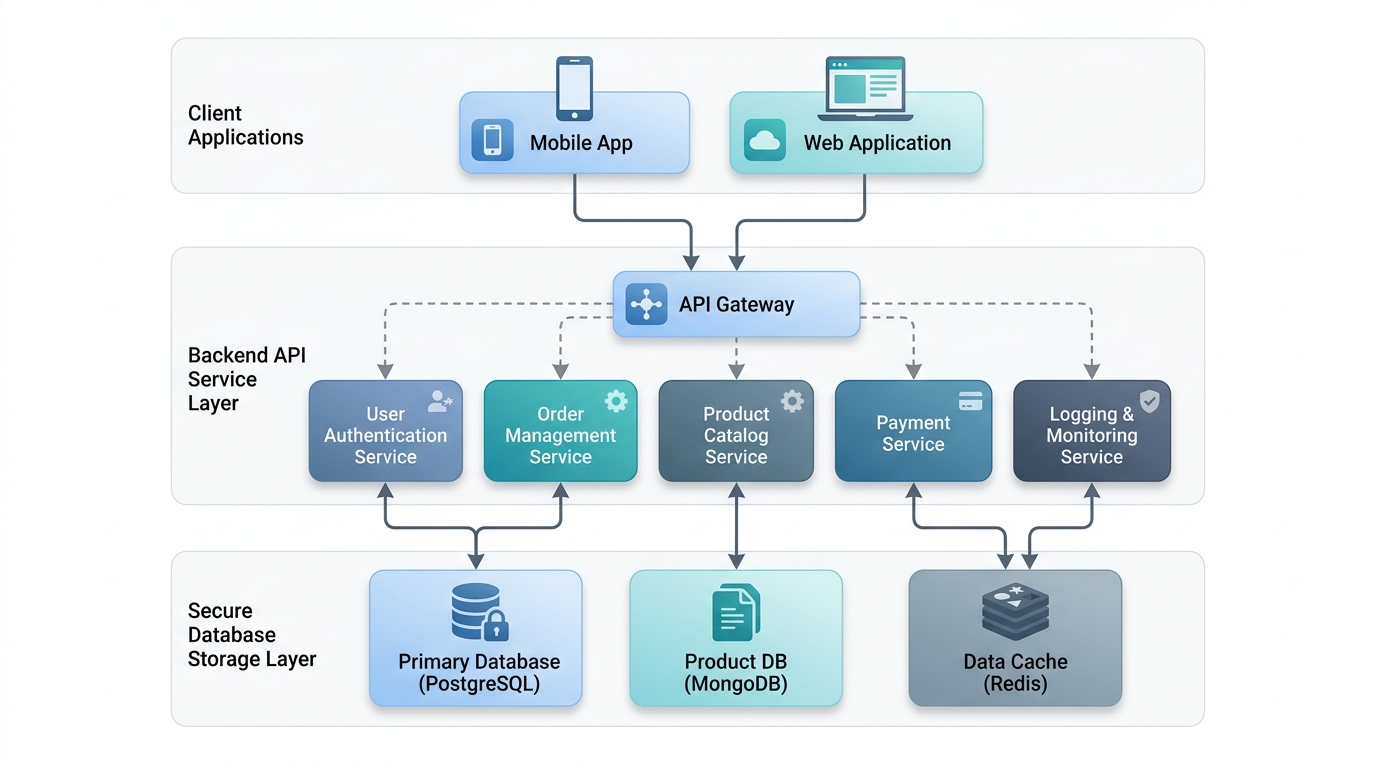
\includegraphics[width=0.75\textwidth]{assets/figuras/ejemplo_figura.png}%
  }{%
    \fbox{\parbox{0.7\textwidth}{\centering\vspace{2cm} [Coloque su figura en assets/figuras/] \vspace{2cm}}}%
  }
  \caption{Esquema conceptual de la arquitectura modular implementada.}
  \label{fig:arquitectura_muestra}
  \fuente{Elaboración propia.}
\end{figure}

\subsubsection{Ejemplo de Bloques de Código Fuente}
Para documentar algoritmos, controladores o esquemas de configuración, utilice el entorno estándar \texttt{lstlisting}:

\begin{lstlisting}[language=Python, caption={Controlador de ejemplo para el procesamiento de solicitudes.}, label={lst:ejemplo_codigo}]
# Controlador modular de ejemplo
class GestionProcesos:
    def __init__(self, repositorio_datos):
        self.repositorio = repositorio_datos

    def registrar_actividad(self, actividad_id: str, detalle: dict) -> bool:
        """Valida y registra una nueva actividad en el repositorio."""
        if not actividad_id or not detalle:
            raise ValueError("Parámetros de actividad inválidos.")
        return self.repositorio.guardar(actividad_id, detalle)
\end{lstlisting}

% =========================================================================
% capitulos/04_conclusiones_recomendaciones.tex
% Secciones Finales: Conclusiones y Recomendaciones
% =========================================================================

\section*{CONCLUSIONES}
\addcontentsline{toc}{section}{CONCLUSIONES}

\subsection*{General}
Presente una conclusión principal que dé respuesta directa al objetivo general planteado en el Capítulo III, destacando el impacto general y el valor técnico aportado a la institución receptora mediante la culminación del proyecto de prácticas preprofesionales.

\subsection*{Específicos}
Redacte una conclusión por cada objetivo específico formulado, demostrando con hechos o métricas su grado de cumplimiento:
\begin{itemize}
  \item Se levantaron y formalizaron los requerimientos técnicos y funcionales del sistema, logrando una comprensión precisa de las necesidades operativas de la entidad receptora.
  \item Se diseñó una arquitectura de software desacoplada y un modelo de datos estructurado, lo cual garantizó la consistencia de la información y la mantenibilidad del código a largo plazo.
  \item Se implementaron los módulos lógicos y servicios web planificados, permitiendo automatizar los flujos de trabajo clave y reduciendo la tasa de errores operativos.
  \item Se ejecutaron las pruebas unitarias y de integración correspondientes, verificando la robustez de los componentes antes de su puesta en marcha en el entorno de pruebas.
\end{itemize}

\clearpage
\section*{RECOMENDACIONES}
\addcontentsline{toc}{section}{RECOMENDACIONES}

Las recomendaciones deben ser propositivas, viables y orientadas a la continuidad o mejora de la labor técnica realizada:

\begin{itemize}
  \item \textbf{A la institución o empresa receptora:} Se recomienda continuar con el plan de actualización tecnológica de la infraestructura restante, así como programar capacitaciones periódicas para el personal usuario de las nuevas herramientas implementadas.
  \item \textbf{Al área técnica de desarrollo:} Se sugiere extender la cobertura de pruebas automatizadas hacia pruebas de estrés y rendimiento, garantizando un comportamiento óptimo ante picos de concurrencia en la plataforma.
  \item \textbf{A la Facultad y Escuela Profesional (UNAS):} Se recomienda seguir incentivando convenios de prácticas preprofesionales con organizaciones que promuevan la aplicación de metodologías de ingeniería y buenas prácticas arquitectónicas.
  \item \textbf{A futuros practicantes:} Se recomienda documentar continuamente los cambios y decisiones técnicas mediante repositorios versionados y estándares de código limpio, facilitando la transferencia de conocimiento entre promociones.
\end{itemize}


% 6. Referencias Bibliográficas (Normas APA)
\clearpage
\bibliographystyle{apalike}
\bibliography{bib/referencias}

% 7. Anexos del Documento
\iniciaranexos
% =========================================================================
% anexos/01_anexos.tex
% Sección de Anexos del Informe
% =========================================================================

\subsection{Especificación Técnica y Diccionario de Datos}
\label{anexo:diccionario_datos}

En este anexo se pueden incluir tablas técnicas extensas, diagramas de base de datos o especificaciones de interfaces que por su extensión no deben interrumpir la lectura del cuerpo principal.

\begin{table}[htbp]
  \centering
  \caption{Estructura representativa de la entidad principal de datos.}
  \label{tab:anexo_entidad_datos}
  \begin{tabularx}{\textwidth}{llLX}
    \toprule
    \textbf{Campo} & \textbf{Tipo} & \textbf{Restricción} & \textbf{Descripción} \\
    \midrule
    \texttt{id} & \texttt{UUID} & Primary Key & Identificador único inmutable del registro. \\
    \texttt{codigo} & \texttt{VARCHAR(20)} & Unique, Not Null & Código administrativo institucional. \\
    \texttt{estado} & \texttt{VARCHAR(15)} & Not Null & Estado operativo (Activo, Pendiente, Inactivo). \\
    \texttt{fecha\_creacion} & \texttt{TIMESTAMP} & Default NOW() & Registro cronológico de auditoría. \\
    \bottomrule
  \end{tabularx}
  \fuente{Elaboración propia.}
\end{table}

\subsection{Guía de Despliegue y Scripts de Automatización}
\label{anexo:scripts_despliegue}

En este anexo se documentan los pasos o fragmentos de código utilizados para el aprovisionamiento de entornos:

\begin{lstlisting}[language=bash, caption={Script de automatización de pruebas y compilación del proyecto.}, label={lst:script_automatizacion}]
#!/usr/bin/env bash
# Script para compilación y verificación automatizada
set -e

echo "Iniciando pruebas unitarias..."
pytest --cov=src tests/

echo "Compilando contenedor de la aplicación..."
docker build -t empresa/sistema-gestion:latest .

echo "Despliegue completado con éxito."
\end{lstlisting}


\end{document}
